	\documentclass[a4paper,12pt, oneside]{book}
	\usepackage[czech]{babel}
	\usepackage[utf8]{inputenc}

	% Pokažené znaky, po Ctrl V z jiného dokumentu
	% umožní najdení znaku, pak smazat
	\DeclareUnicodeCharacter{202F}{FIX ME!!!!}

	% Plugin na sloupce
	\usepackage{multicol}

	\usepackage{wrapfig}

	% Zdroje a reference
	\usepackage[
	  backend=biber,        % if we want unicode and many other features (biber is already by default)
		  style=iso-numeric, % or another iso-<style>
	]{biblatex}

		\addbibresource{refs.bib}

	% Zobrazování kodu
	\usepackage{listings}

	\usepackage{xcolor}

	% Plugin na obrazky
	\usepackage{graphicx}

	% Toto je plugin diky kteremu pujde klikat do obsahu
	\usepackage{hyperref}
	\hypersetup{
		colorlinks,
		citecolor=black,
		filecolor=black,
		linkcolor=black,
		urlcolor=blue
	}

	% Plugin na hezci nadpis kapitoly
	% https://texblog.org/2012/07/03/fancy-latex-chapter-styles/
	\usepackage[T1]{fontenc}
	\usepackage{titlesec, blindtext, color}
	\definecolor{gray75}{gray}{0.75}
	\newcommand{\hsp}{\hspace{20pt}}
	\titleformat{\chapter}[hang]{\Huge\bfseries}{\thechapter\hsp\textcolor{gray75}{|}\hsp}{0pt}{\Huge\bfseries}



	% Zakladni info o dokumento
	\title{Zálohování a ochrana před ransomwarem}
	\def\topic{Zálohování a ochrana před ransomwarem}
	\def\schoolclass{Oktáva}
	\author{Lukáš Dulík}
	\date{\today} % Tady sa pak moze nastavit jine datum, ted to da vzdycky aktualni

	% Vytvoření proměnných, které budou přístupné z celého dokumentu
	\makeatletter
	\let\newtitle\@title
	\let\newauthor\@author
	\let\newdate\@date
	\makeatother


	% Plugin na zahlavi zapati
	\usepackage{fancyhdr}


	% Záhlaví a zápatí
	\fancyhf{}
	\lhead{\topic}
	\lfoot{Maturitní práce \schoolclass}
	\rfoot{\thepage}

	% Dulezite pro spravne zobrazovani zahlavi zapati
	\pagestyle{empty}
	\fancypagestyle{plain}{}



	% Zobrazování kódu
	\definecolor{codegreen}{rgb}{0,0.6,0}
	\definecolor{codegray}{rgb}{0.5,0.5,0.5}
	\definecolor{codepurple}{rgb}{0.58,0,0.82}
	\definecolor{backcolour}{rgb}{0.95,0.95,0.92}

	\lstdefinestyle{codestyle}{
		backgroundcolor=\color{backcolour},   
		commentstyle=\color{codegreen},
		keywordstyle=\color{magenta},
		numberstyle=\tiny\color{codegray},
		stringstyle=\color{codepurple},
		basicstyle=\ttfamily\footnotesize,
		breakatwhitespace=false,         
		breaklines=true,                 
		captionpos=b,                    
		keepspaces=true,                 
		numbers=left,                    
		numbersep=5pt,                  
		showspaces=false,                
		showstringspaces=false,
		showtabs=false,                  
		tabsize=2
	}	

	\lstset{style=codestyle}





	\begin{document}

% Zrusi cislovani na zacatecnich strankach
\pagenumbering{gobble}

\begin{titlepage}
    \begin{center}
        \vspace*{1cm}

        \Large
		Gymnázium Jana Pivečky a Střední odborná škola Slavičín \\

		% Logo GJP
		
\includegraphics[width=0.4\textwidth]{img/gjp.png}

		\Huge \textbf{\topic}

        \vspace{0.5cm}
        \Large
        Maturitní práce

    \end{center}
	\vspace{0.7cm}
	\vspace{0.7cm}

	\makeatletter
	\begin{normalsize}
	\null\hfill%
	\begin{tabular}{p{3cm} p{7cm} }
		Předmět: & Informatika \\
		Vypracoval: & \@author \\ 
		Školní rok:	& 2024/2025 \\
		Třída: &	\schoolclass \\
		Studijní obor:	& 7941K/81 Gymnázium	\\
		Vedoucí práce:	& Mgr. Michal Botek \\
		Oponent:	& Mgr. Ladislav Jurča 
	\end{tabular}
\end{normalsize}
	\vspace{0.5cm}
	\vfill

	

	\Large

	\begin{center}
		Slavičín 2025
	\end{center}


	\makeatother

	\vspace{5pt}


\end{titlepage}

\newpage


\noindent

Prohlašuji, že tato závěrečná maturitní práce je mým původním autorským dílem,
které jsem vypracoval samostatně. Všechny zdroje, prameny a literaturu, které
jsem při vypracování používal nebo z nich čerpal, v práci řádně cituji
s uvedením úplného odkazu na příslušný zdroj.

\begin{center}
Ve Slavičíně

% Proměnná s dnesnim datem
\newdate

\vspace{10mm}

% Proměnná s autorem dokumentu
\newauthor
\end{center}

\newpage
\section*{Abstrakt}

Cílem této práce je popsat proces návrhu a realizace jednoduchého
systému pro zálohování dat. Výsledný systém má sloužit pro zabezpečení důležitých
dat prostřednictvím pravidelného zálohování.

Základem navrženého zálohovacího systému je jednodeskový počítač Rasp\-berry Pi 5,
ke kterému je pro ukládání záloh připojen pevný disk pomocí USB
dokovací stanice. Pro ochranu a integraci těchto komponent byl navržen a
vytištěn na 3D tiskárně speciální držák. 

Důležitým znakem tohoto provedení byla snaha o využití existujících
hardwarových prostředků. Konkrétně se jednalo o komponenty, které již nebyly
aktivně používány a nacházely se v domácích zásobách.

Tento přístup nejenže snížil finanční náročnost projektu, ale také umožnil
prozkoumat možnosti opětovného využití starší technologie pro nové účely.

Realizace byla úspěšná a zálohovací systém se podařilo zprovoznit. Systém
vykazuje rychlosti až 30 MB/s, což je pro vlastní účely adekvátní. Celkově 
se cíl práce podařilo splnit.

\newpage
\section*{Poděkování}

Děkuji vedoucímu práce Michalu Botkovi za konzultace týkající 
se psaní této práce. 

% Udela obsah
\tableofcontents

\clearpage
% Zacatek cislovani stranek
\pagenumbering{arabic}
\pagestyle{fancy}

\chapter{Úvod}

Často opomíjené, ale v počítačových systémech nutné - to je zálohování.
Mnozí z nás uchovávají data na svém vlastním uložišti. Ať už to jsou
fotky z dovolených nebo cenné pracovní dokumenty, mají pro nás vysokou hodnotu, a proto 
o ně nechceme přijít. Máte vytvořenou zálohu svých dat? 

Lidé jsou zvyklí ukládat svá data na USB disky. Ruční zálohování má však své limity,
proto se pojďme podívat na způsob, jak dělat zálohování poctivě.


\section{Vlastní motivace}

Motivací pro napsání této práce byla nutnost vytvoření zálohy mého
domácího PC. Uchovávám na něm mnoho cenných dat -
jedná se asi o 1 TB fotek a videí. Tato data mám na HDD, které
slouží již 10 let. Je na konci své životnosti a já nechci přijít o data,
která na něm uchovávám. 

Dalším důvodem byl také fakt, že ransomwarové útoky jsou stále častější. Míří
jak na státní instituce, tak na firmy a domácnosti. To přináší další rizika pro
moje data. Proto jsem se rozhodl vytvořit funkční systém 
pro zálohování.


% TODO: Ransomware


\section{Cíle projektu}

Cílem projektu bylo vytvořit systém pro zálohování počítačových dat. Moje
požadavky pro zálohovací systém byly následující: 

\begin{enumerate}
	\item Automatizace - zálohy se vytváří automaticky ve stanovených intervalech
	\item Nízká cena - co nejmenší počáteční i provozní náklady
	\item Spolehlivost - systém nevykazuje chyby
	\item Transparentnost - můžu sledovat průběh zálohování
	\item Error handling - chybové záznamy jdou jednoduše přečíst
\end{enumerate}

V dalších kapitolách zhodnotíme, jestli se tyto
požadavky podařilo splnit.


\section{Cloud vs On-Premise}

Na trhu je mnoho cloudových řešení pro zálohování. Ať už to jsou známé služby
jako Google Drive a OneDrive, nebo levnější alternativa v podobě Back\-blaze
Backup, cloudové společnosti poskytují spolehlivé řešení pro potřeby zálohování.
Cena těchto služeb je však vysoká a pro moje účely nevýhodná. 

Kvůli vysoké ceně jsem se rozhodl vytvořit vlastní hardwarové řešení na
zálohování (On-Premise).
Následující kapitoly popisují
proces výběru hardwaru, způsob připojení disku, návrh držáku a softwarovou
konfiguraci systému. 


\chapter{Hardware}
\section{Volba platformy}

Co vlastně potřebujeme za platformu? Stačí nám počítač, který bude 
schopný fungovat jako NAS server. Takový server nepotřebuje velký
výpočetní výkon, můžeme tak využít i mikropočítače. 


\subsection{Raspberry Pi 5}

Jde o nejnovější verzi slavného mikropočítače, který má v sobě čtyřjádrový ARM
procesor. Tuto desku jsem již vlastnil, byla pro mě tedy jasným favoritem.
Nakonec jsem ji použil právě pro tento projekt. Její spotřeba je opravdu nízká
a pohybuje se kolem 3 Wattů v nečinnosti.  \cite{RPi-Power}

\begin{figure}[h]
	\centering
	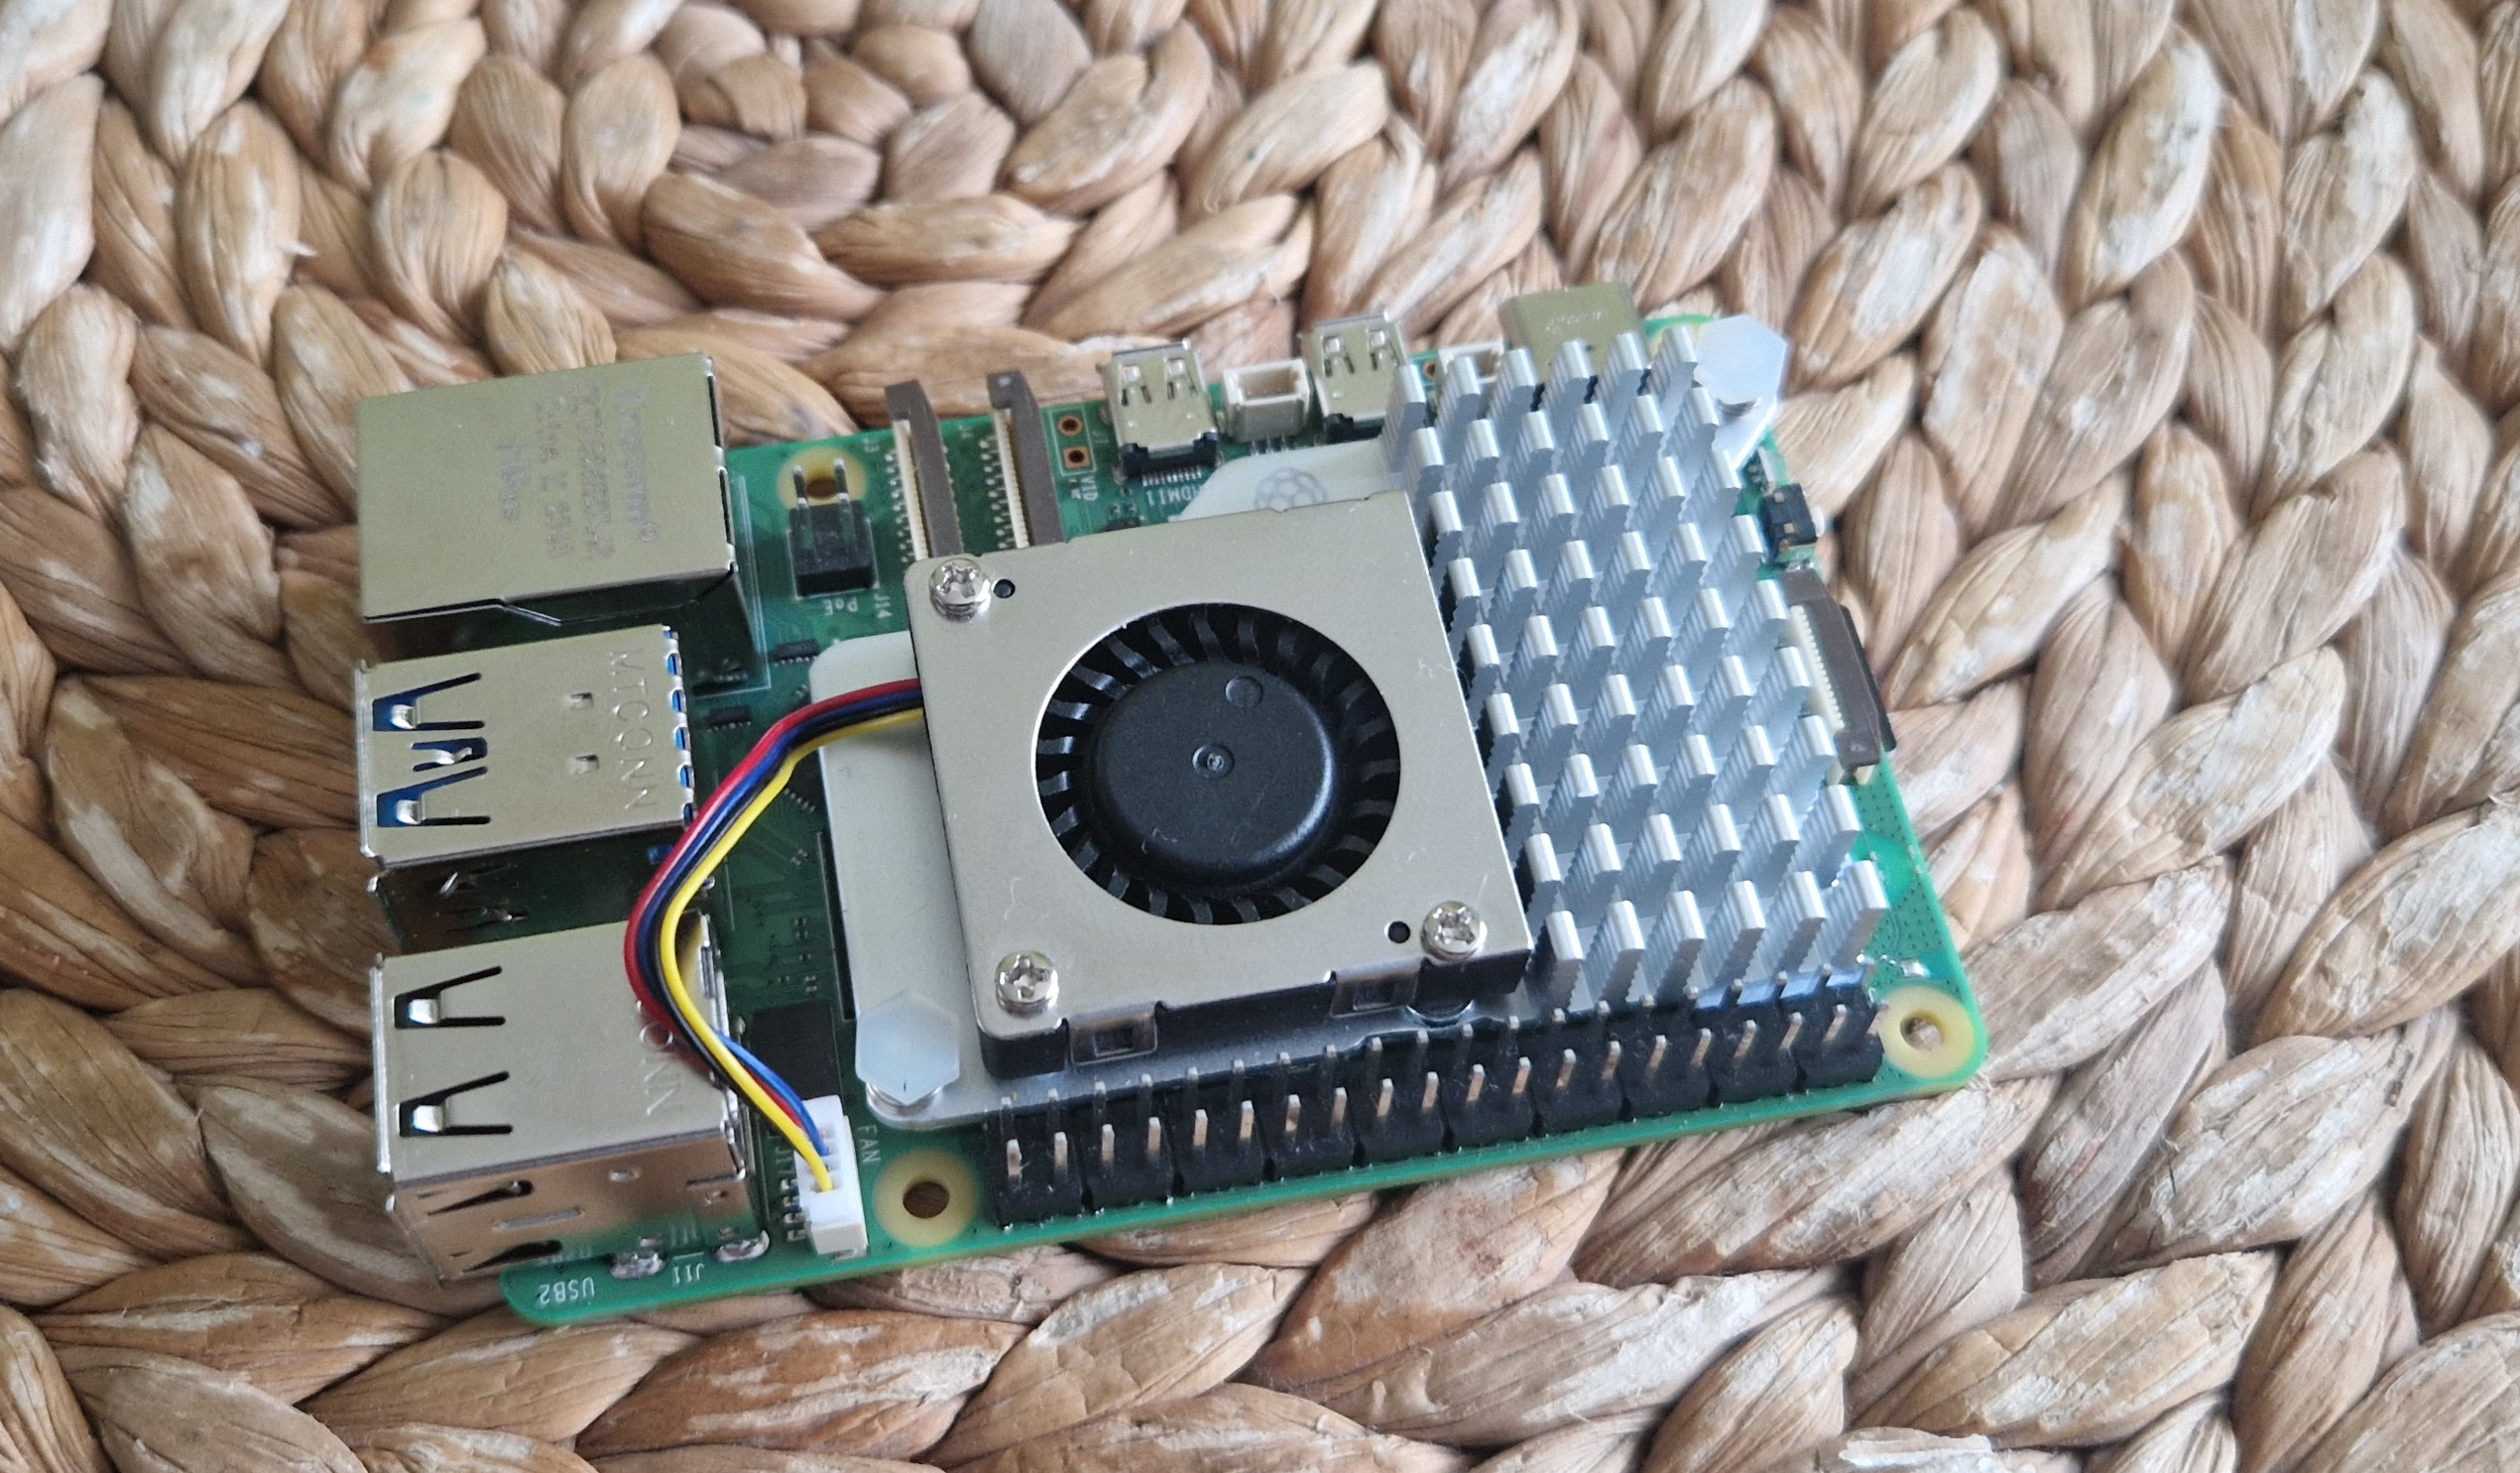
\includegraphics[width=0.6\textwidth]{img/rpi5-active-cooler-c.jpg}
	\caption{RPi 5 s aktivním chladičem}
\end{figure}

\subsection{Server x86}

Rackové servery tradičního slova smyslu jsou pro projekty tohoto typu
více než vhodné. Zkušenosti se servery tohoto typu
jsem nasbíral na brigádách v lokálním ISP UnArtel. 

\subsection{NAS zařízení}

Komerční NAS zařízení, jako například od společností Synology a QNAP, nabízejí
uživatelsky přívětivé řešení pro síťové ukládání dat. Kdybych 
měl na starost zálohování firemních dat, možná bych sáhnul po komerčních
produktech. Očekával bych, že budou vysoce spolehlivé a nenáročné na obsluhu.
Nicméně pro moje účely se toto řešení nehodí. Roli hraje jak vysoká cena,
tak nízká vzdělávací hodnota při použití již existujícího řešení.

\subsection{Závěr}



Na základě výše uvedených úvah jsem se rozhodl pro svůj zálohovací systém použít
platformu Raspberry Pi 5. Hlavním důvodem byla jeho dostupnost, což přímo
naplňuje požadavek na nízké náklady. Dalším významným faktorem byla příležitost
k získání praktických zkušeností s konfigurací hardwaru a softwaru při stavbě
vlastního řešení.


\section{Jak připojit disk k RPi 5?}

Nevýhoda Raspberry Pi je absence SATA rozhraní pro připojení disků.
Musel jsem tak sáhnout po alternativním řešení v podobě 
USB-to-SATA adaptéru značky AXAGON. Tato česká značka nabízí 
velký sortiment příslušenství tohoto typu. Doma nám ležel v šuplíku
USB HDD Dock této značky, jehož využití pro mě 
bylo jasnou volbou.

\begin{figure}[h]
	\centering
	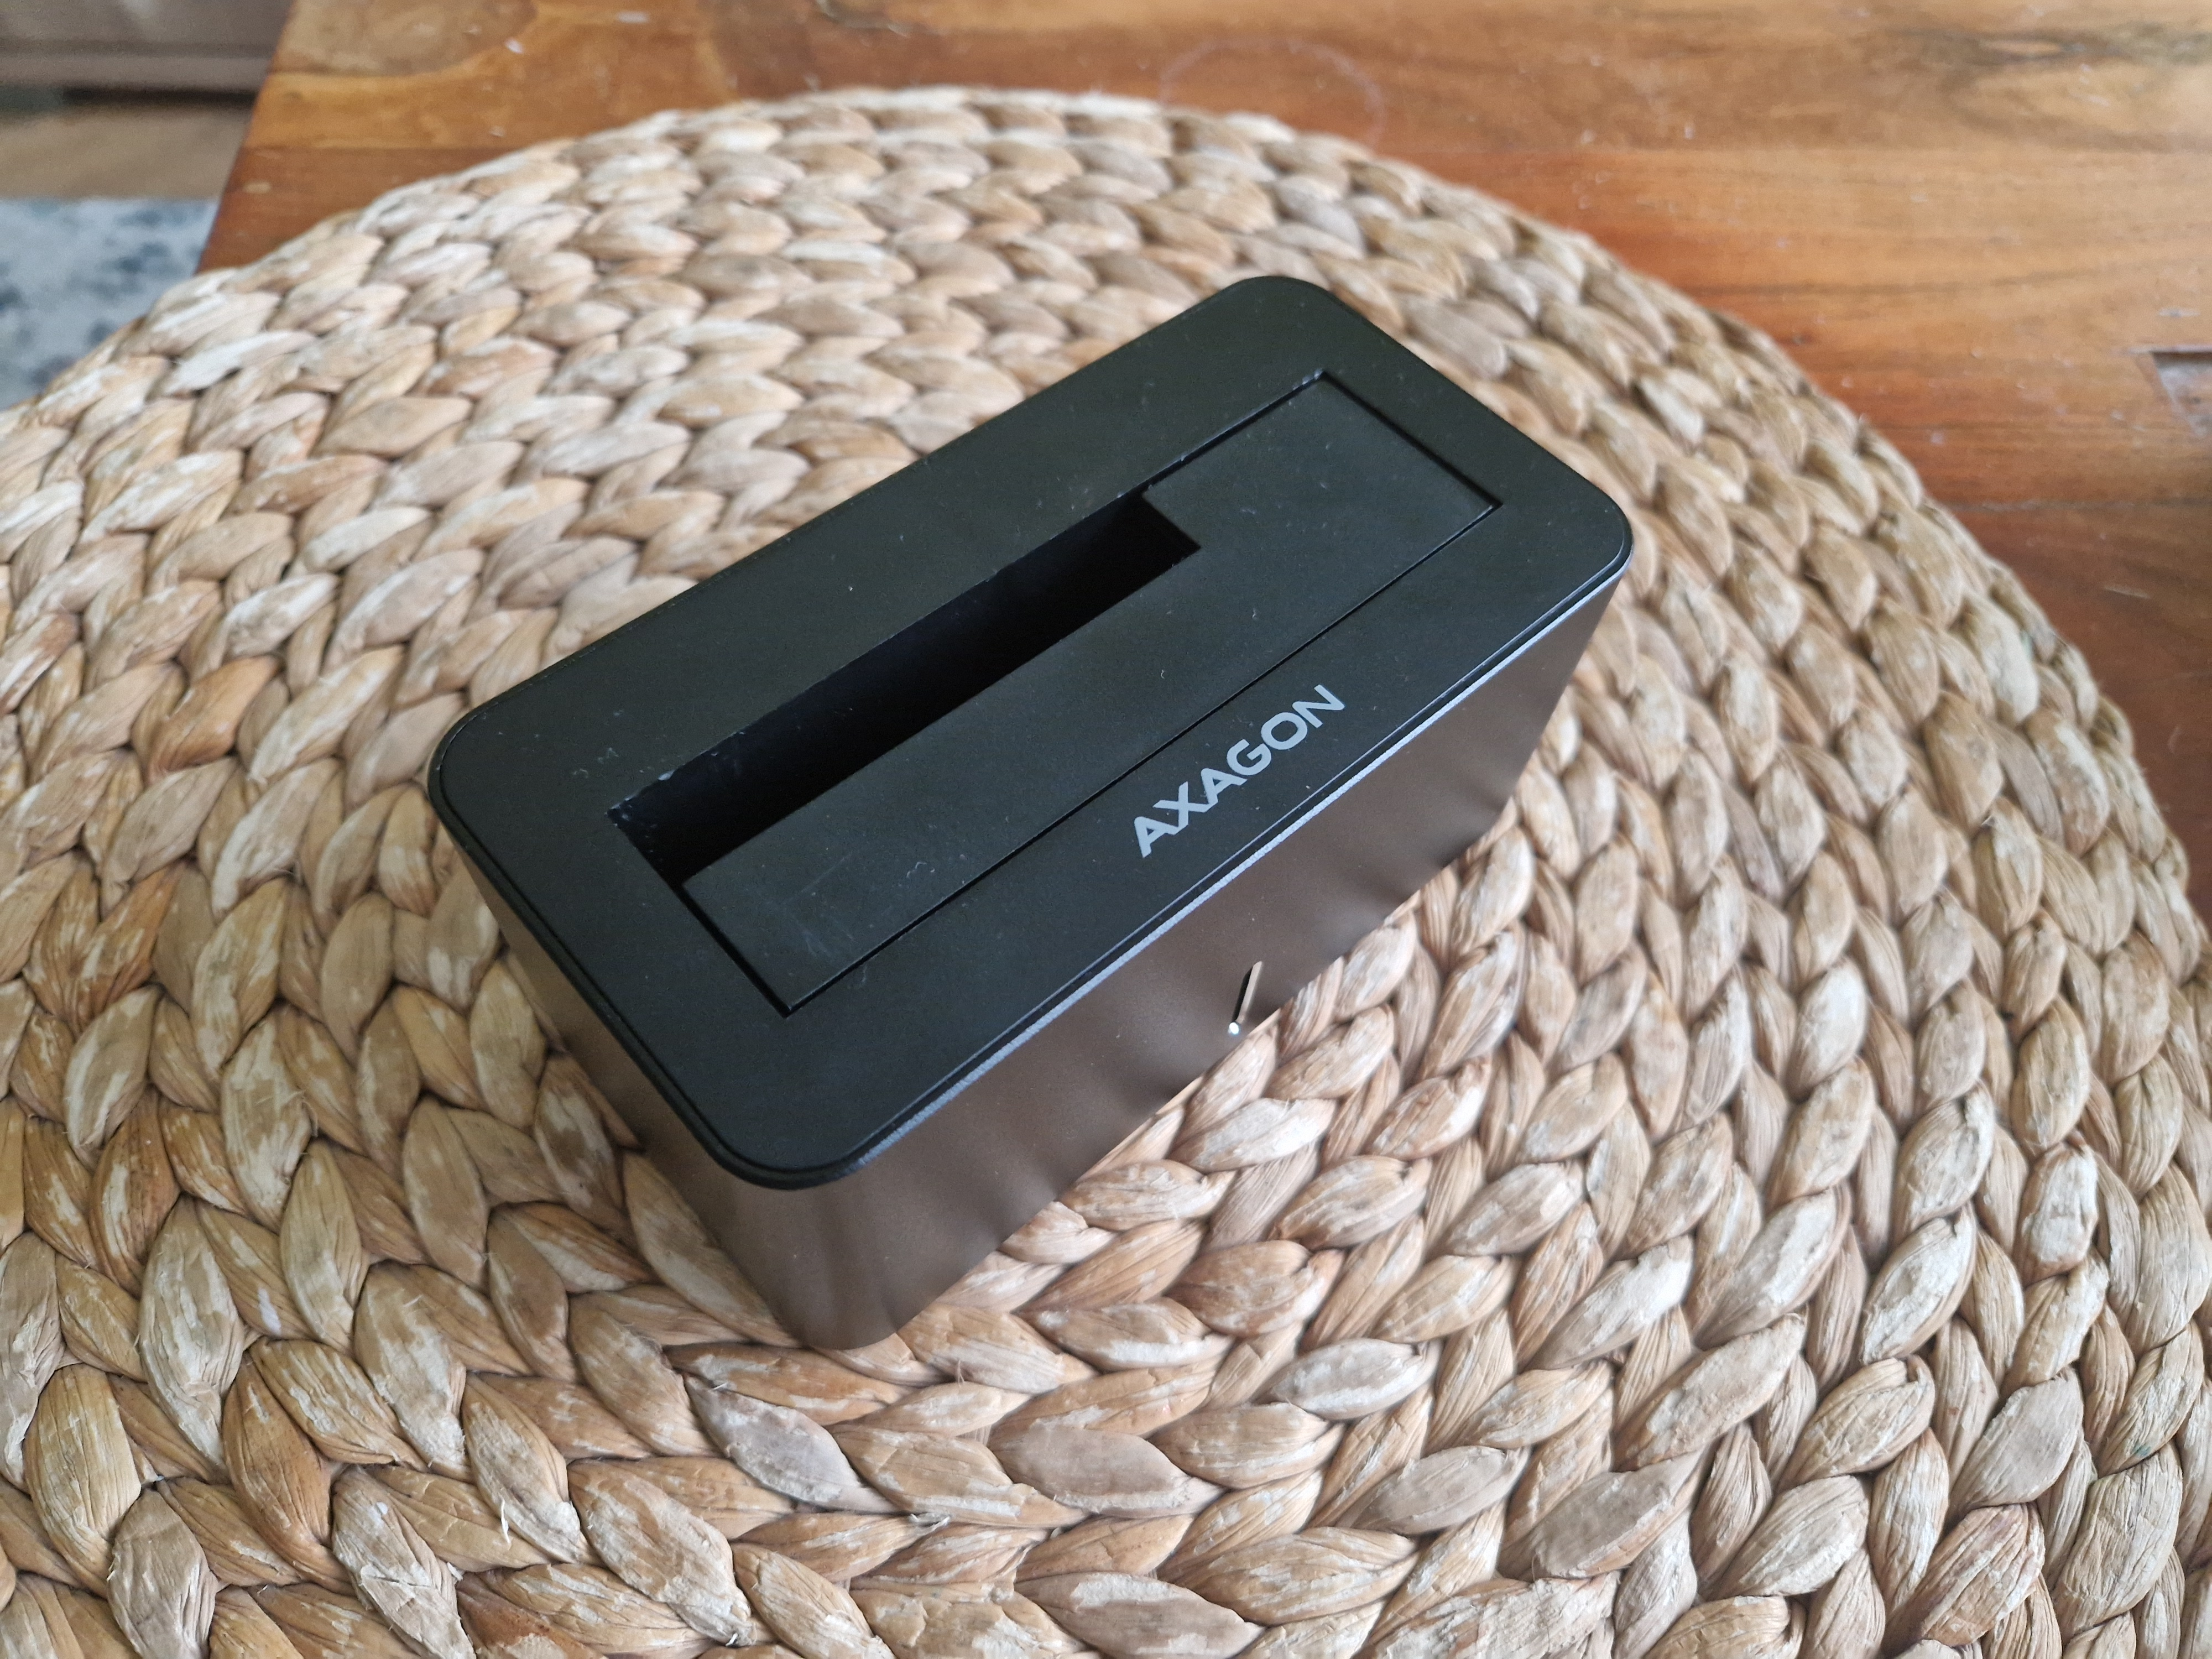
\includegraphics[width=0.4\textwidth]{img/axagon.jpg}
	\caption{USB HDD Dock \href{https://www.axagon.eu/produkty/adsa-sn}{AXAGON ADSA-SN}}
\end{figure}

Nejprve jsem ale musel vyzkoušet, jestli je tento dock kompatibilní 
s Raspberry Pi. Ukázalo se, že je připojení bezproblémové, a tak
jsem mohl začít testovat použité 2TB disky pocházející ze serverů
firmy UnArtel. Spouštěl jsem testy S.M.A.R.T. pomocí programu smartctl.

\begin{lstlisting}
smartctl -t short /dev/device
\end{lstlisting} 

Vypadalo to beznadějně, všechny disky vykazovaly vady. 
Naštěstí jsem ale našel jeden disk, který fungoval bezproblémově.
Připojil jsem ho k Raspberry Pi a pomocí nástroje
\emph{fdisk} jsem ho formátoval a vytvořil nové oddíly.
Poté jsem příkazem \emph{mkfs.ext4} vytvořil nový souborový systém.




\section{3D tištěný kryt}

Především kvůli ochraně před poškozením obvodů jsem se rozhodl 
sestrojit vlastní kryt. K návrhu jsem použil CAD software 
Autodesk Fusion 360, k němuž mám jako student přístup zdarma.
Hlavním cílem bylo spojit komponenty do jednoho celku.


\begin{figure}[h]
\centering
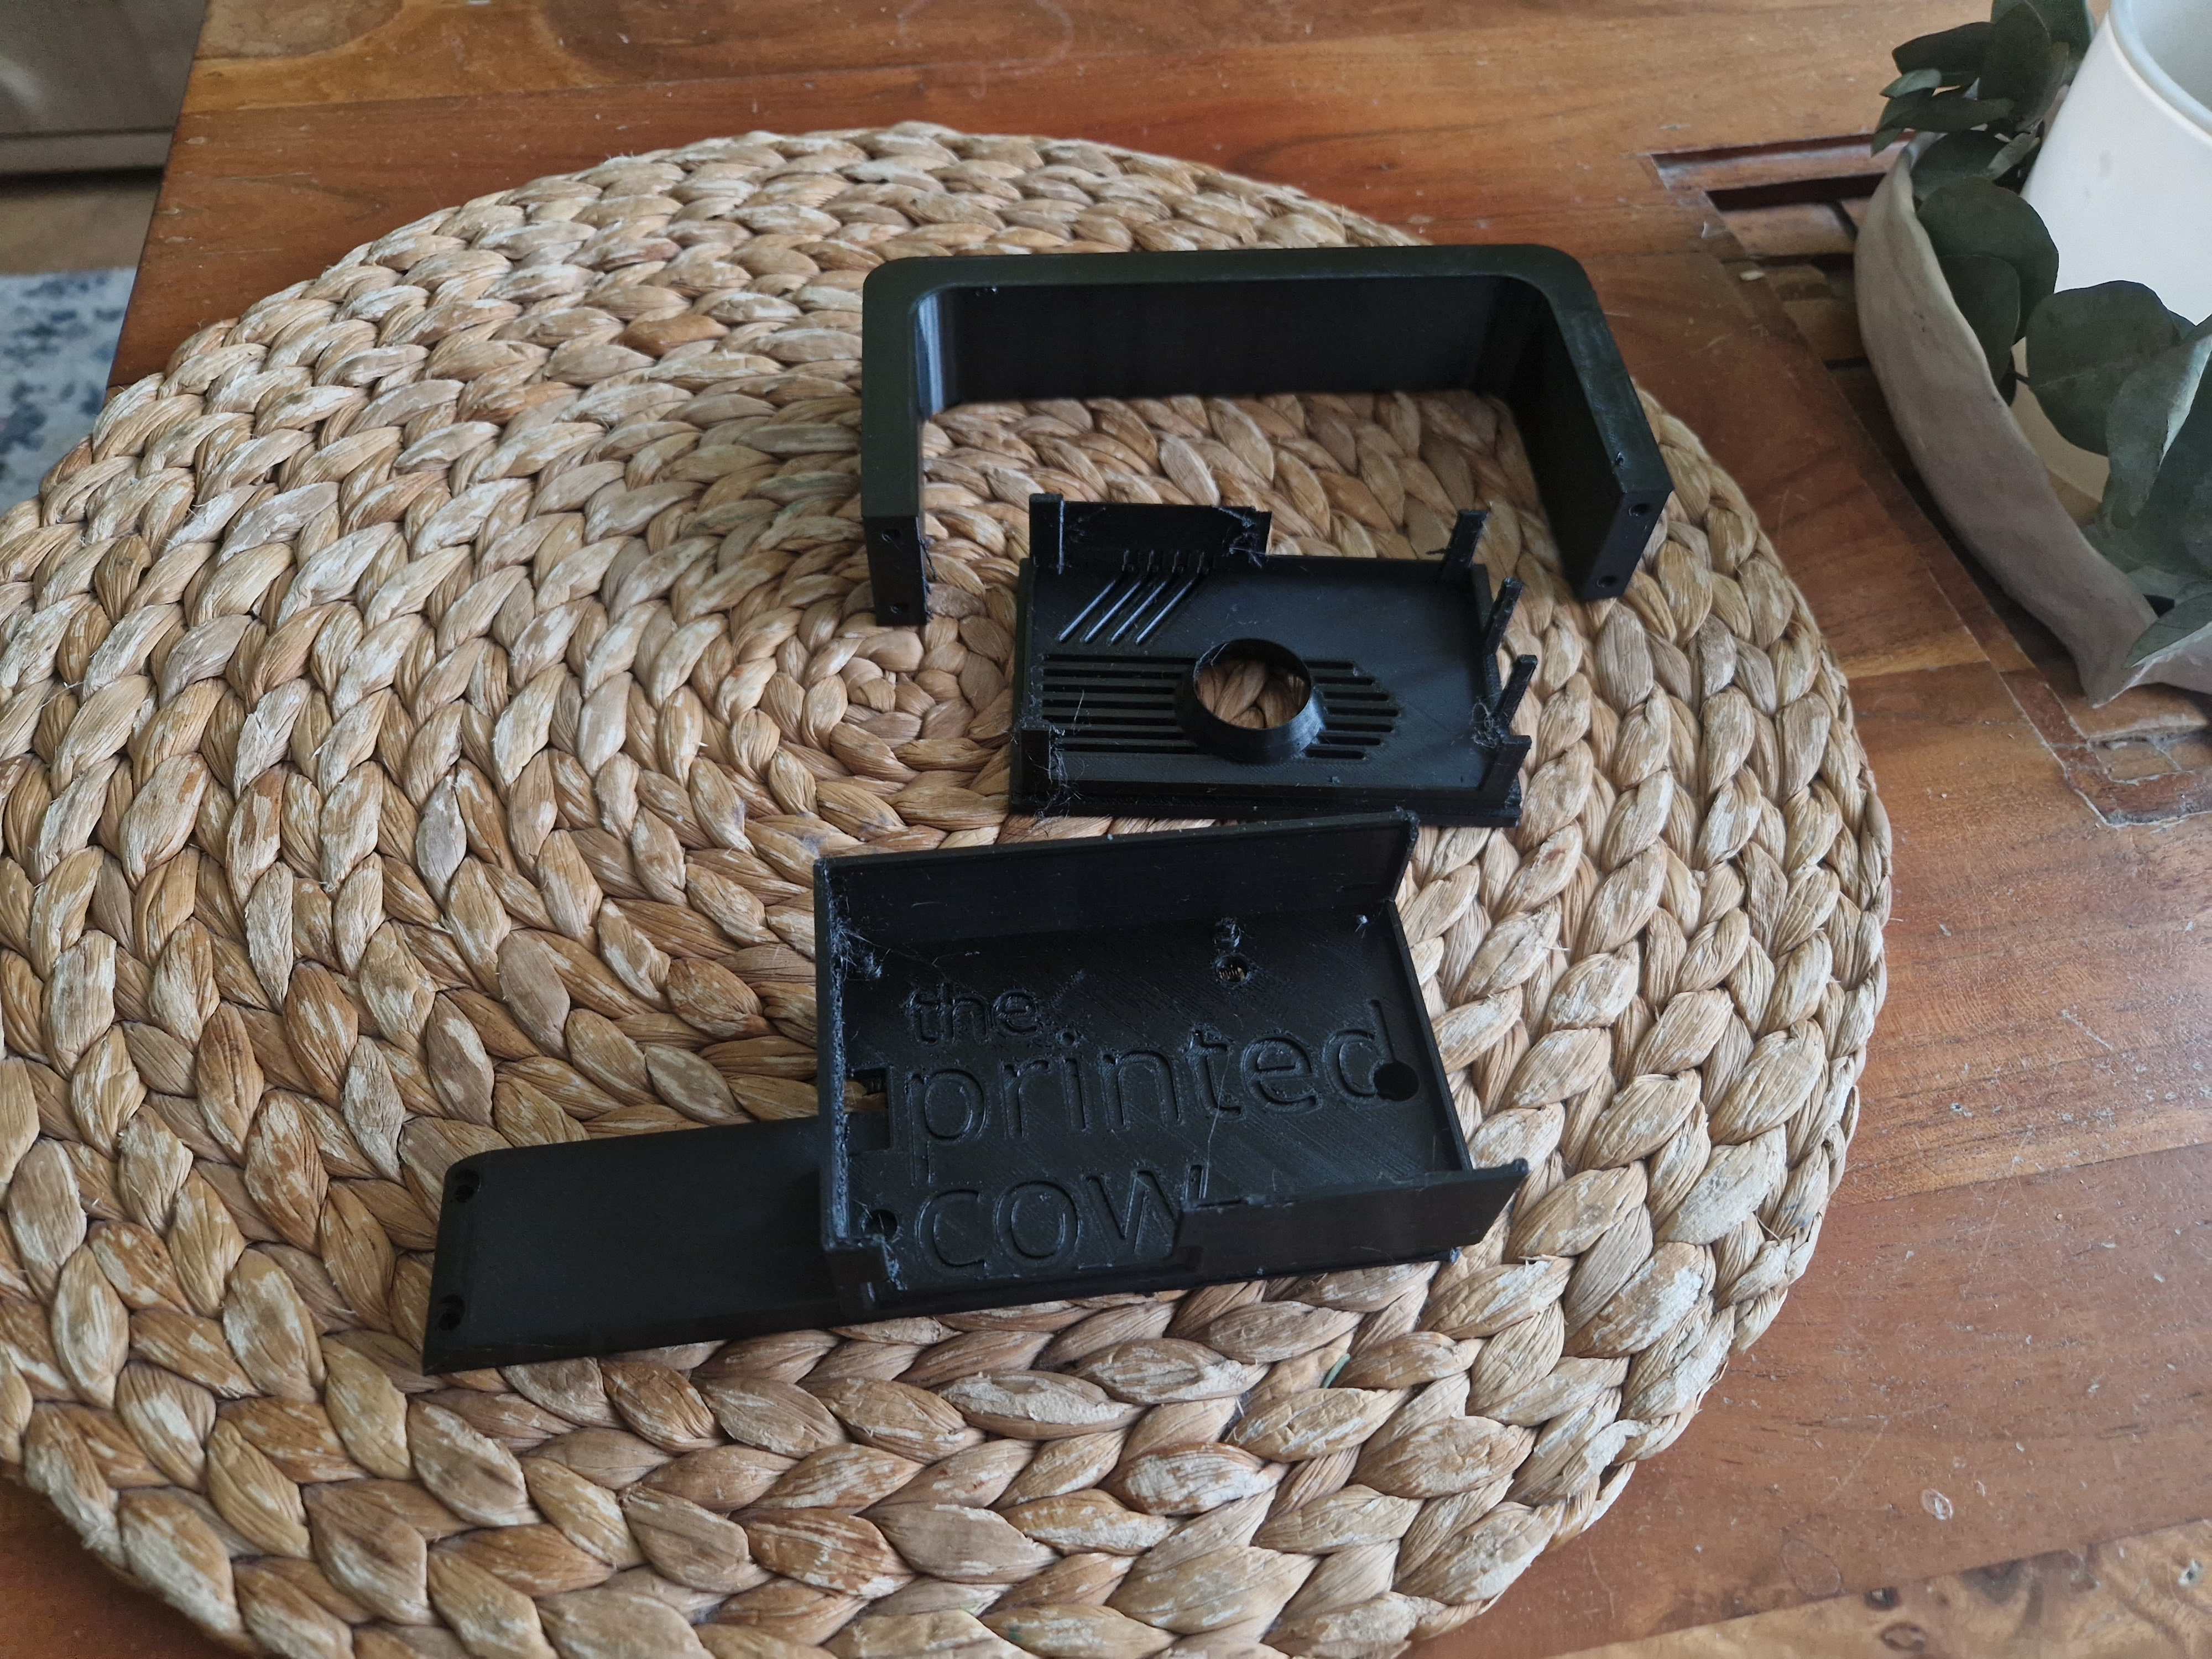
\includegraphics[width=0.8\textwidth]{img/dily-zvlast.jpg}
\caption{Díly vytištěné na 3D tiskárně}
\end{figure}

Důležitým prvkem návrhu je objímka, která pevně drží USB dokovací stanici.
Skládá se ze dvou dílů, které jsou spojeny šrouby M3. Jeden z dílů jsem
spojil s
\href{https://www.printables.com/model/705427-retro-raspberry-pi-5-case-snap-fit}{krytem
na Raspberry Pi}, který jsem našel na internetu.

\begin{figure}[h]
	\centering
	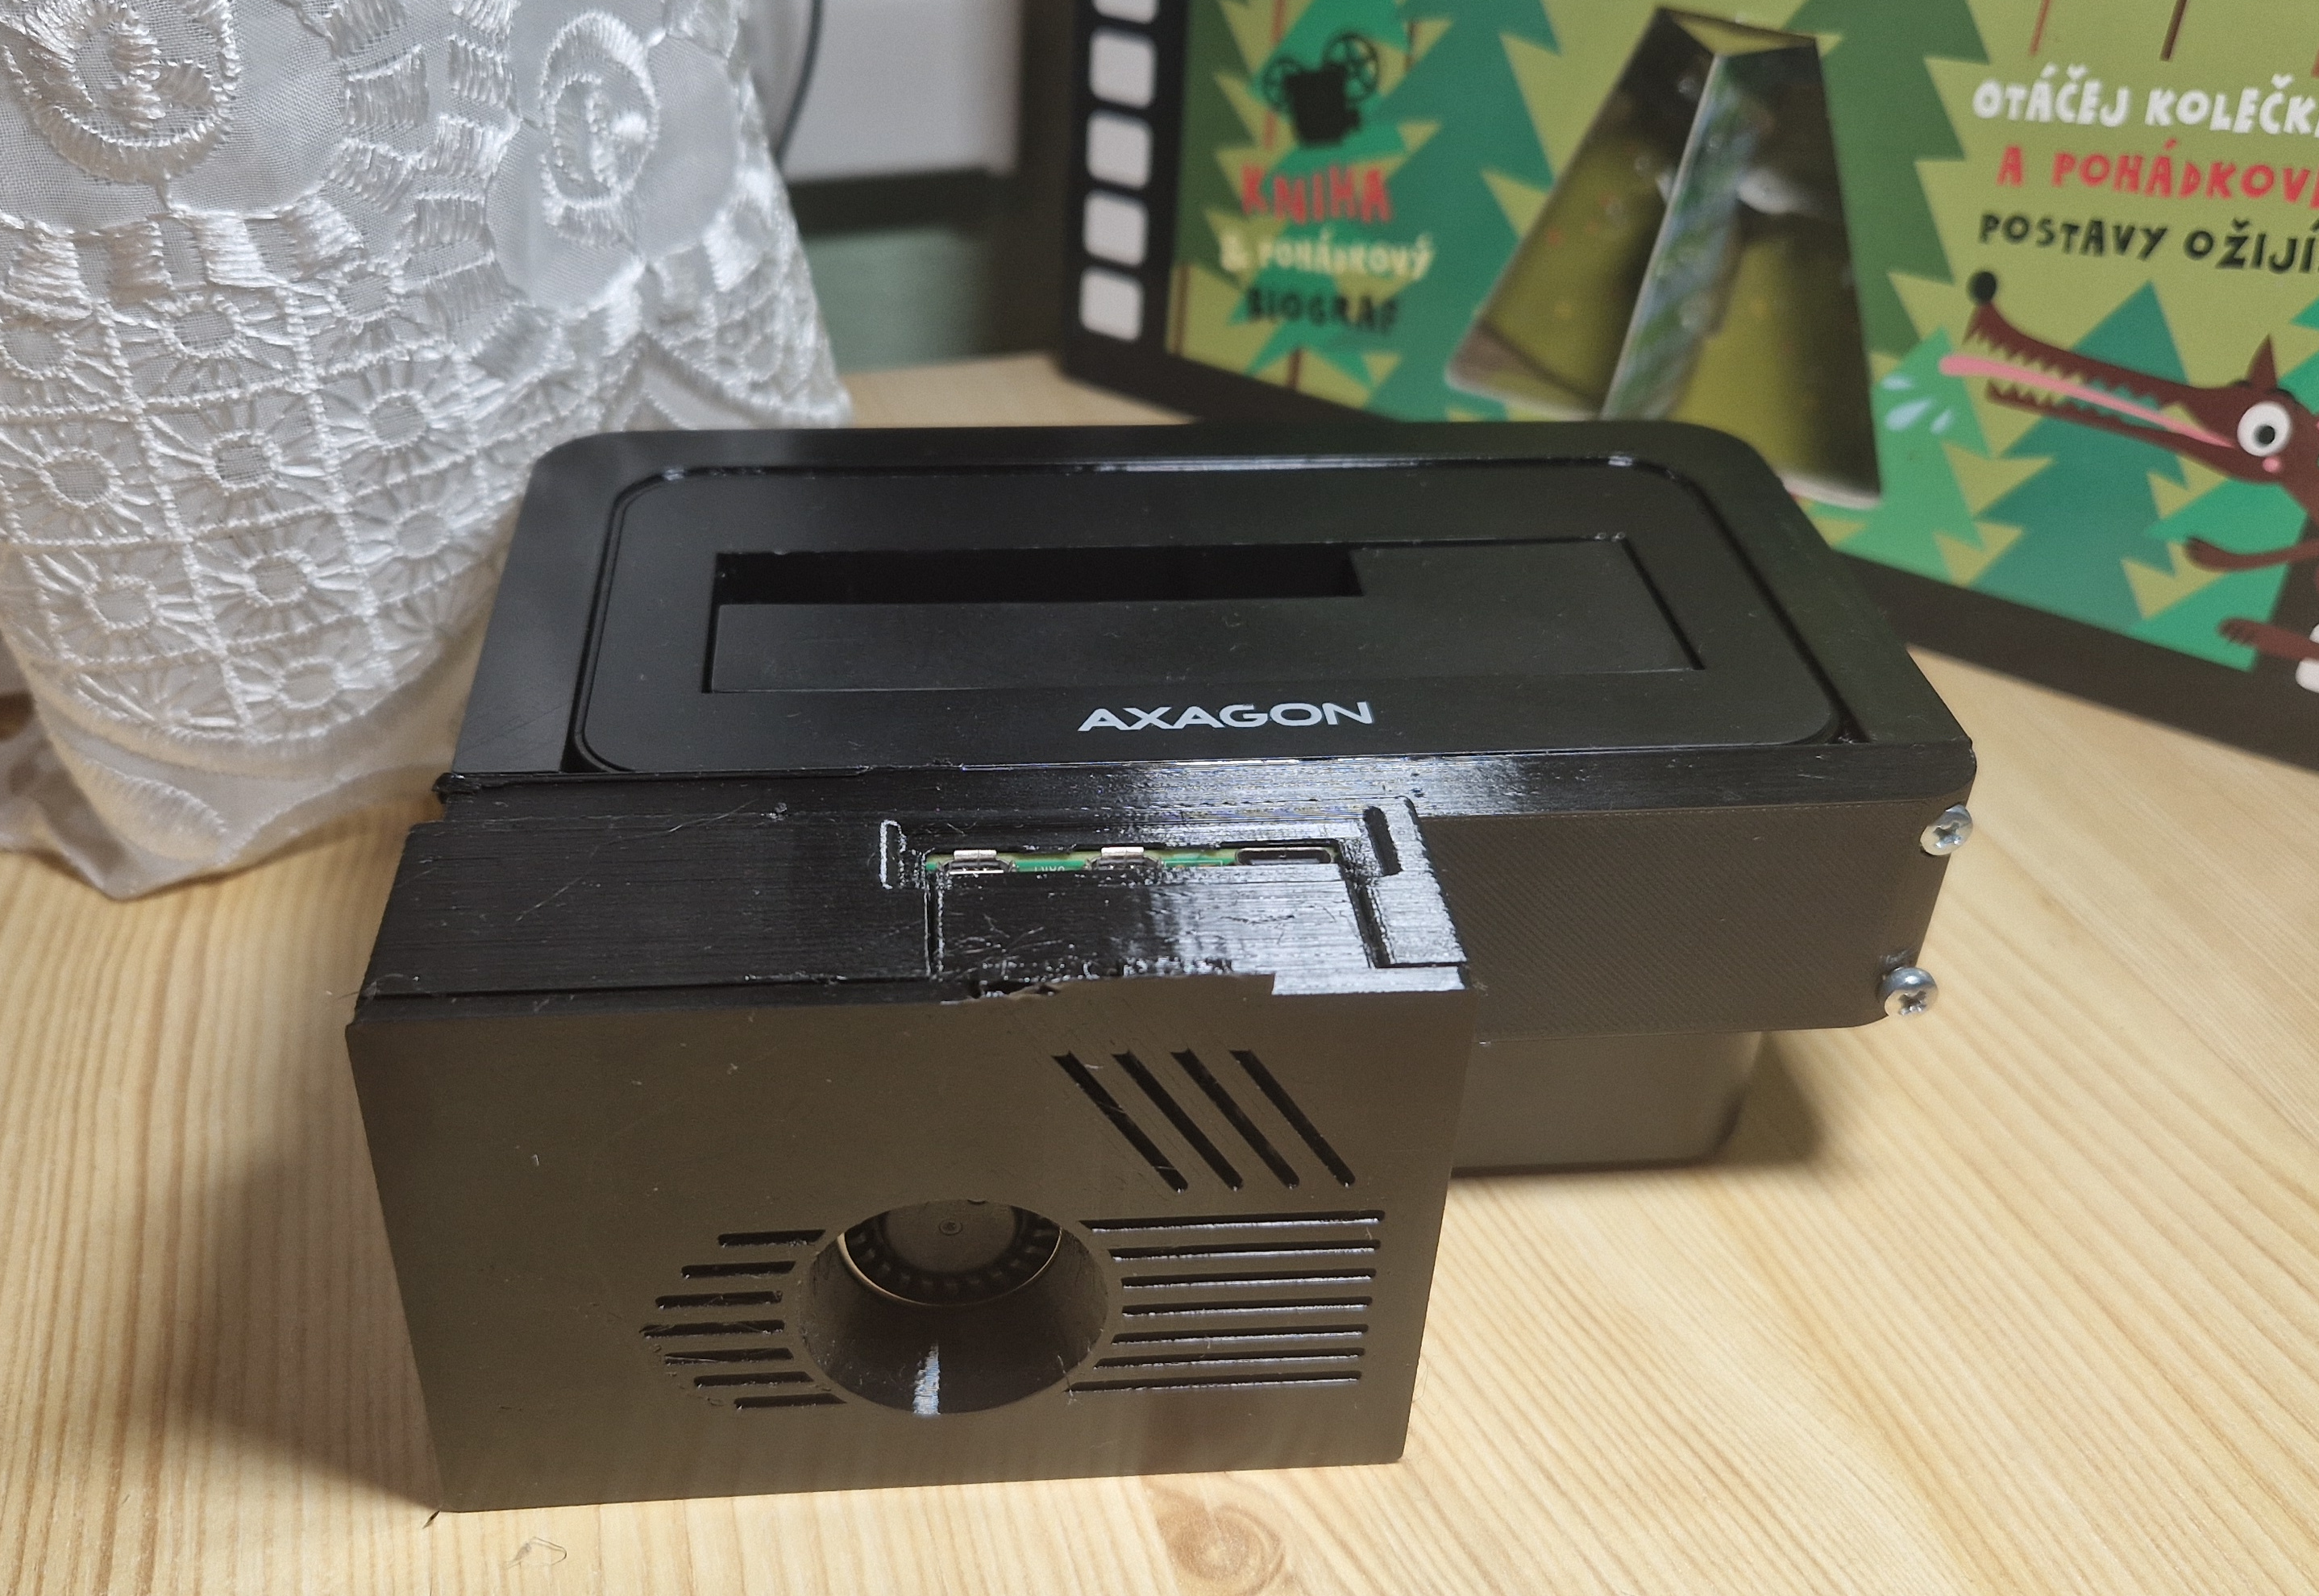
\includegraphics[width=1\textwidth]{img/skladani4-c.jpg}
	\caption{Sestavená zálohovací stanice}
	\end{figure}


Po sestavení těchto dílů vypadalo celé zařízení velmi esteticky. 
Podařilo se mi totiž napodobit tvar objímky i její barvu.
Problém nastal až v momentě, kdy jsem propojil jednotlivé komponenty. 
To přineslo kabelový chaos, který se mi zatím nepovedlo vyřešit.

Hotové zařízení jsem zapojil v serverovně UnArt, díky čemuž bude 
záloha uložena mimo domov jako off-site backup.



\begin{figure}[h]
\centering
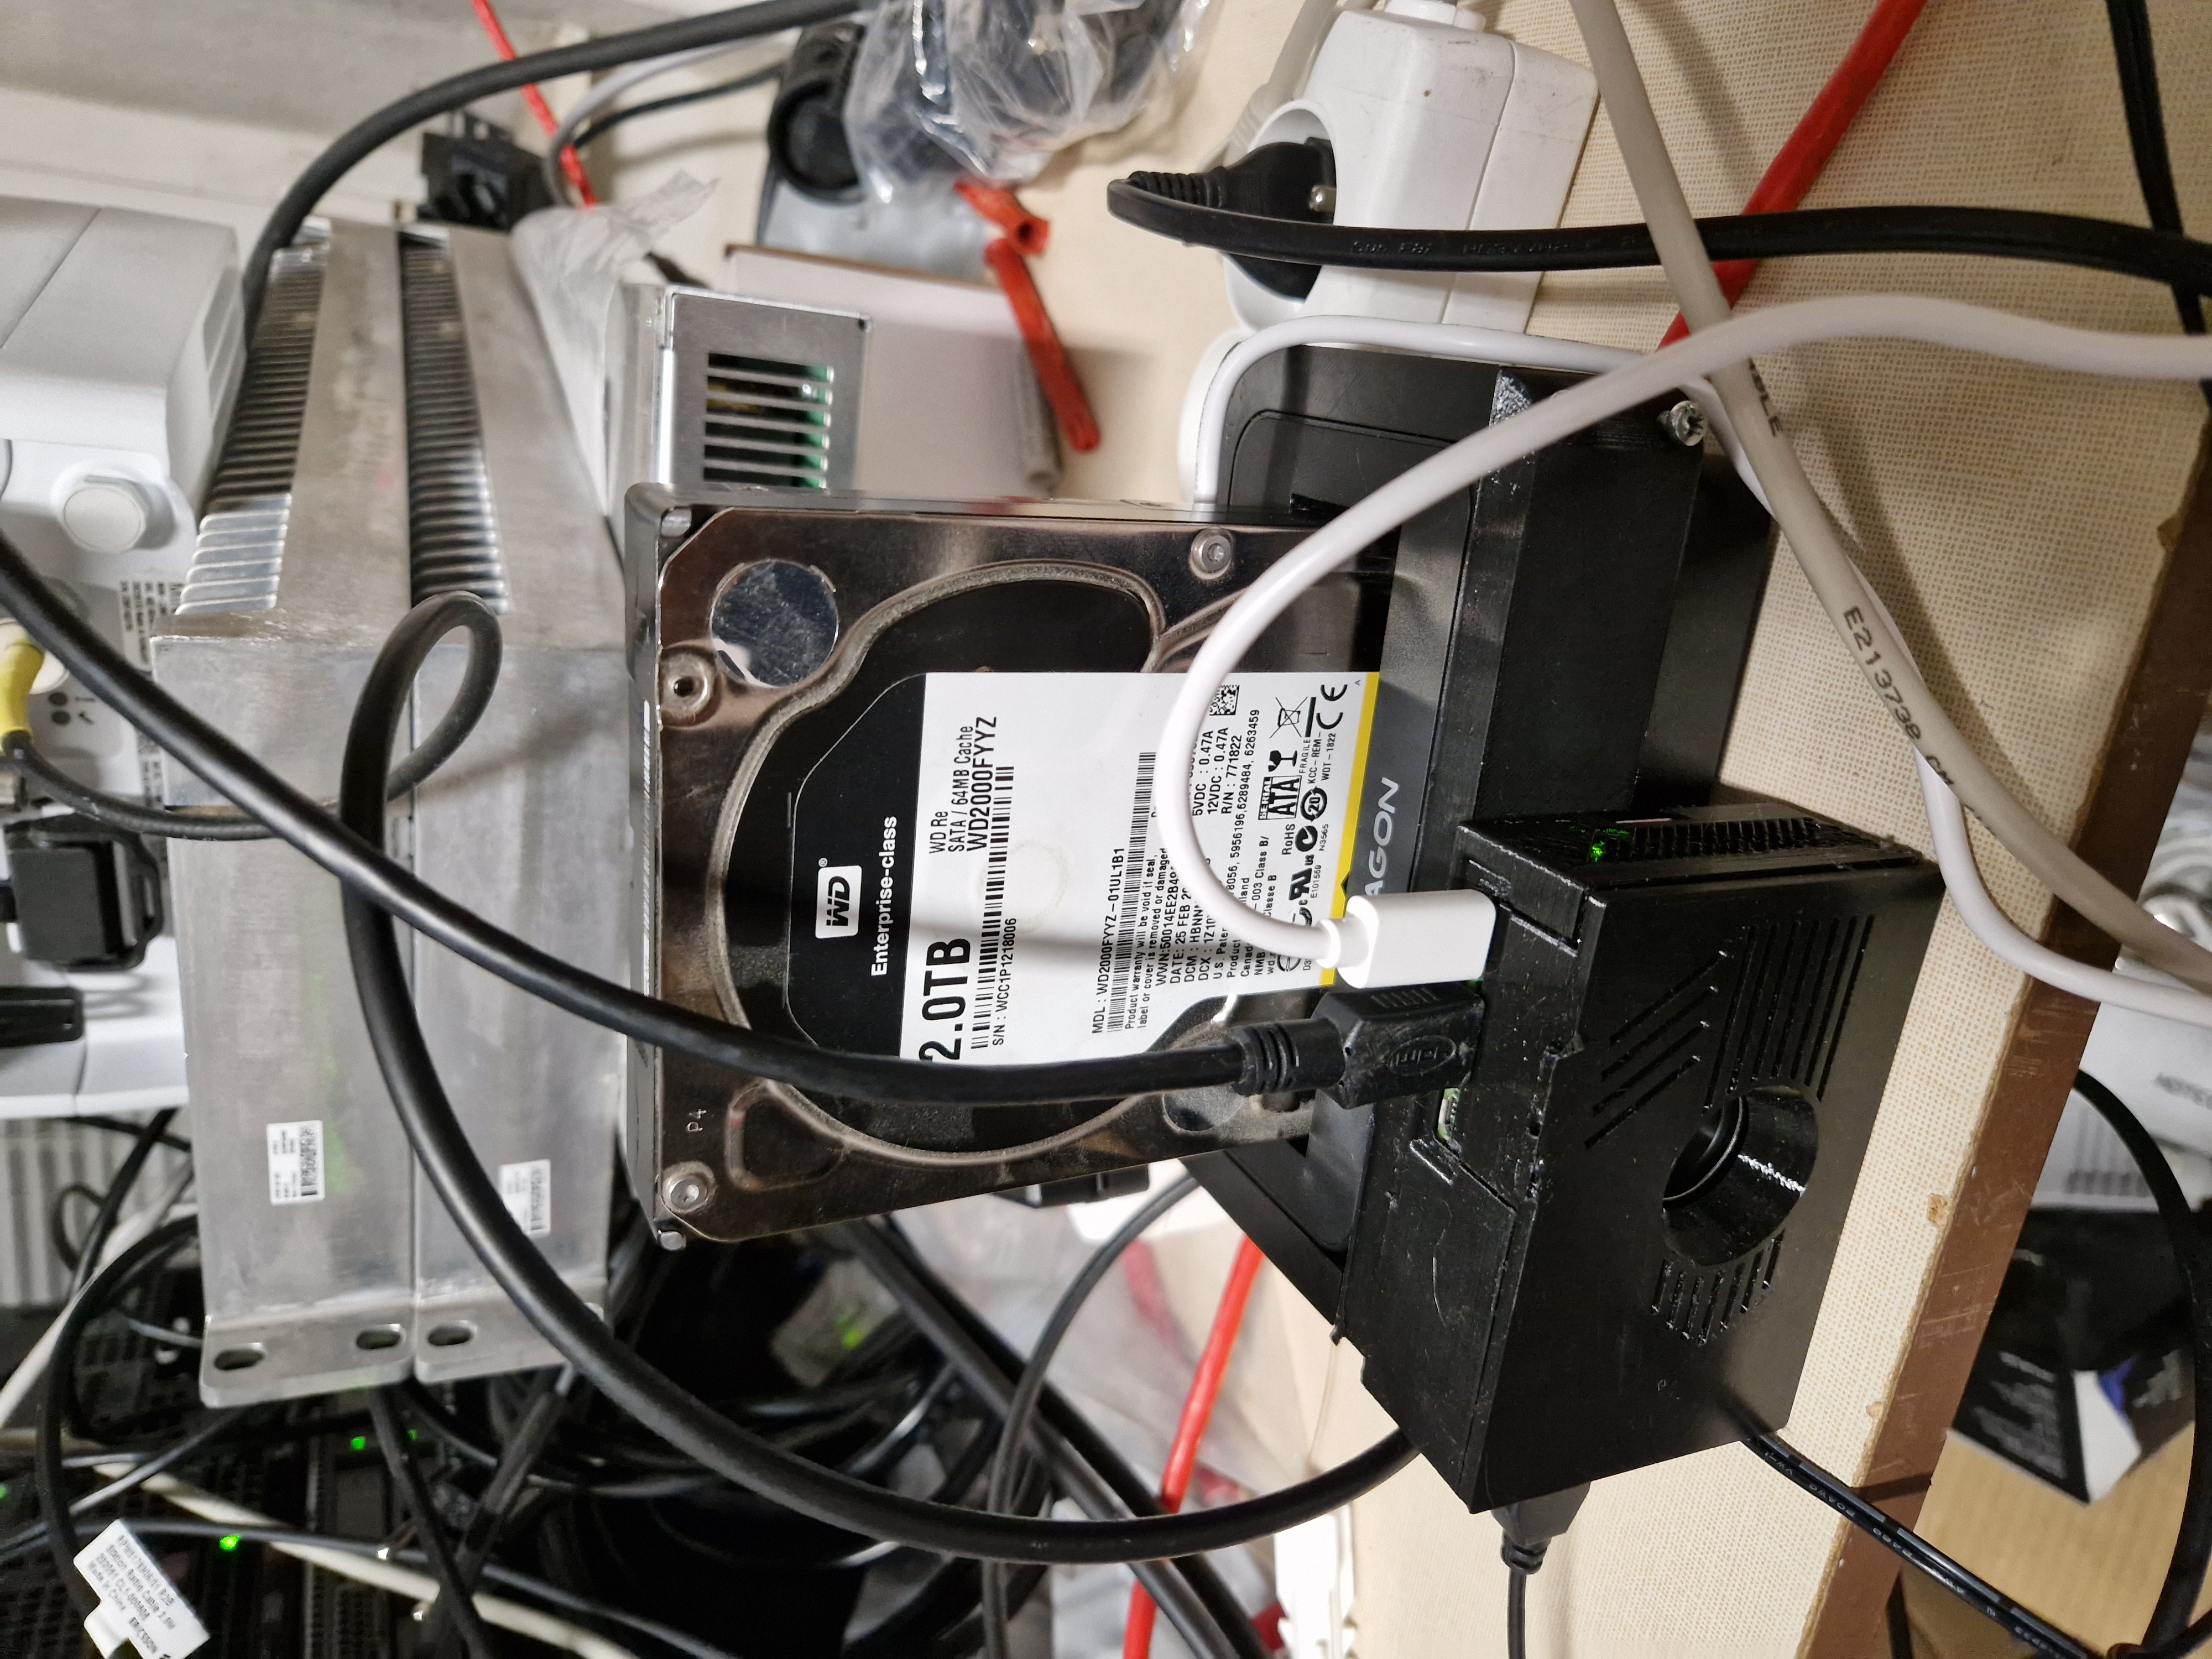
\includegraphics[width=0.9\textwidth]{img/zapojeni4.jpg}
\caption{Připojení všech komponent včetně disku}
\end{figure}


% TODO: kabely

% Umístnění UnArtel, Gigabit

\chapter{Software}

\section{Vzdálené připojení}

Po připojení RPi k internetu jsem se k němu připojil přes SSH, 
abych ho mohl ovládat na dálku. OpenSSH server jsem zabezpečil zakázáním
\emph{Password\-Authentication} v konfiguračním souboru. K RPi se tak přihlašuji  
veřejným klíčem. 

Z mého domácího PC přistupuji k souborům na disku RPi pomocí SFTP.
Tento protokol funguje nativně se serverem OpenSSH, a tak jsem už nemusel
nic konfigurovat.

\section{Správa zálohování}
Pro správu zálohování bylo potřeba vybrat vhodný software. 
Zvažoval jsem několik open-source řešení jako například 
Kopia, BorgBackup nebo Duplicati. Nakonec jsem vybral software 
Kopia. 

\begin{wrapfigure}{r}{0.4\textwidth}
	\centering
	
\includegraphics[width=0.4\textwidth]{img/kopia.jpg}
	\caption{Logo Kopia}
\end{wrapfigure}

Kopia je moderní nástroj, který vznikl v dílně Jarka Kowalského, 
programátora z Googlu. Používá jazyk Go a je velmi dobře optimalizovaný.
\cite{Kopia-GitHub}
Zálohy jsou vytvářeny ve formě inkrementálních snapshotů,
což znamená, že se po opakovaném spuštění nevytváří nová záloha, ale 
připíšou se pouze změny a nově přidané soubory. Podporuje deduplikaci,
díky čemuž je vícero kopií jednoho souboru ukládáno pouze jednou. 
Zálohy jsou automaticky komprimované a šifrované, takže se nejen ušetří 
místo, ale také jsou data uložena bezpečně. \cite{Kopia-Docs} Zato však hlavním
tahákem pro mě byla podpora cloudu. Těší mě, když vím, že v případě vyčerpání
místa na 
zálohovacím HDD můžu v Kopia změnit repozitář a začít tak zálohovat na 
Google Drive.
Kopia má celou řadu dalších výhod,
které jsou popsány v dokumentaci na \url{https://kopia.io/docs/}.

\begin{figure}[h]
\centering
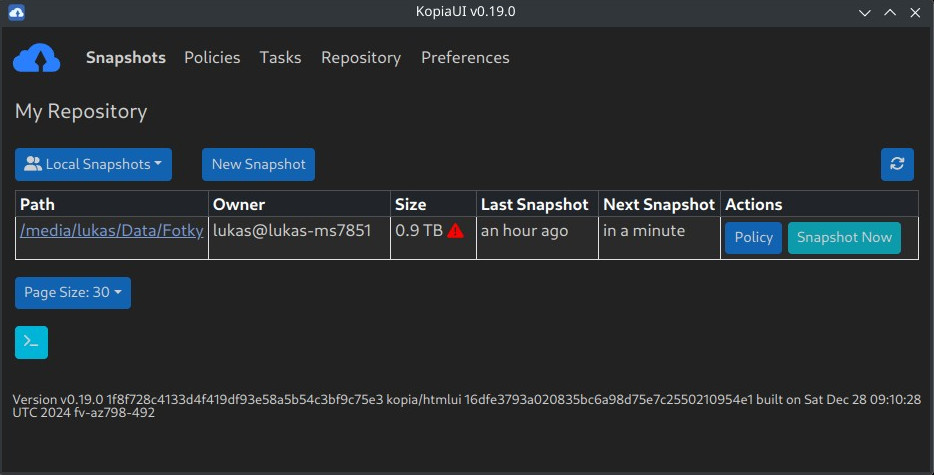
\includegraphics[width=1\textwidth]{img/kopiaUI-Snapshots.jpg}
\caption{Rozhraní KopiaUI}
\end{figure}


\section{Konfigurace Kopia}

Po instalaci Kopia na mém domácí PC jsem mohl začít
konfigurovat. Kopia má jednoduché a uživatelsky přívětivé CLI rozhraní, které
obsahuje příkazy pro vytvoření zálohovacího repozitáře (místo, kde jsou ukládány
zálohy) i pro vytvoření samotných snapshotů. Postrádá však funkce pro
naplánování zálohování. Ke konfiguraci jsem tak použil grafické rozhraní
KopiaUI, které má v sobě funkce pro automatické spouštění zálohování ve
stanovených intervalech. 

\begin{figure}[h]
\centering
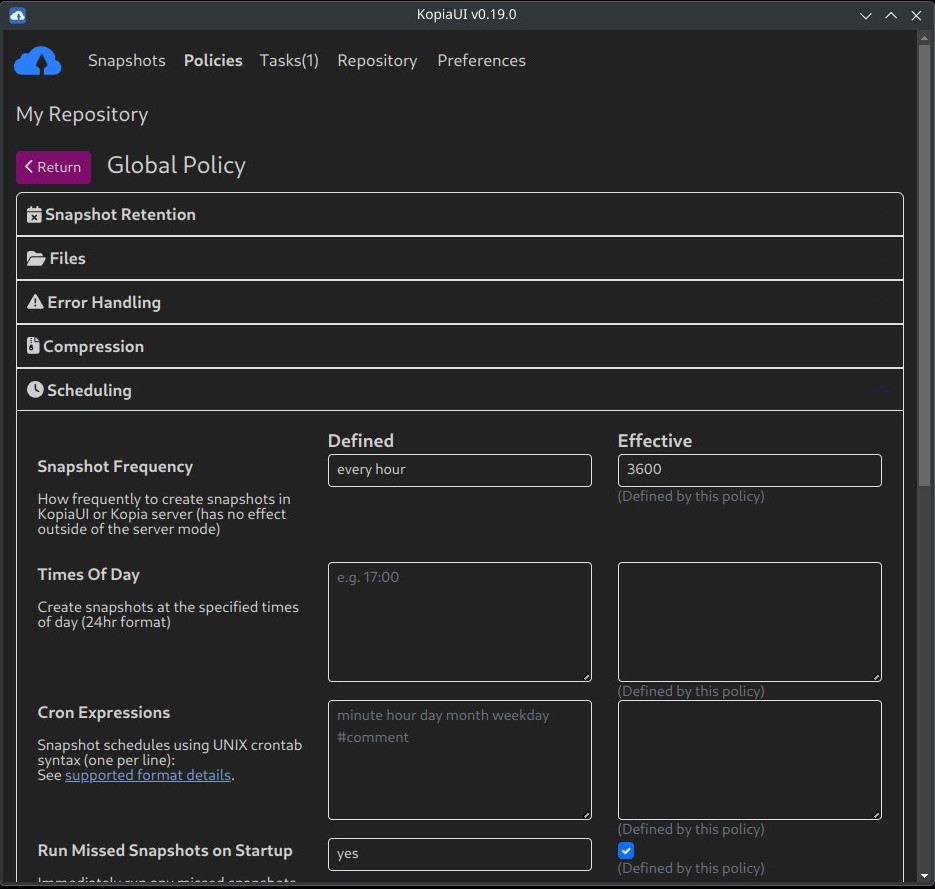
\includegraphics[width=1\textwidth]{img/kopiaUI-Policy.jpg}
\caption{Nastavení frekvence zálohování v KopiaUI}
\end{figure}

\newpage

\section{První snapshot}

Když jsem poprvé spustil zálohování, byl jsem ohromen, jakou rychlostí se 
snapshot tvořil. Rychlosti dosahovaly až 30 MB/s. V KopiaUI jsem viděl průběh
zálohování i logy, ve kterých by se zobrazily případné chyby. Požadavky 
na transparentnost byly tak rovněž splněny.

\newpage

\section{Výpočetní náročnost}

Při vytváření snapshotu je CPU v mém PC zatíženo na 70 \%. Ačkoliv
počítač stále reaguje a dá se na něm pokračovat v práci, jedná se o vysokou
hodnotu. Vyšší náročnost na CPU je způsobena především funkcemi pro šifrování, kompresi
a deduplikaci, které Kopia využívá. 

Druhým důvodem je slabý výkon mého CPU. Jde o Intel Pentium G3258.
Tento procesor byl vydán v roce 2014 a má pouze dvě jádra. 

Ve výsledku mi ale vyšší výpočetní náročnost nevadí. 
Algoritmy, které Kopia využívá, jsou podle mého názoru velmi dobře
optimalizované. V praxi to znamená, že vytvoření snapshotu 1 TB složky, ve které
nebylo nic změněno, trvá 30 sekund. Výpočetní čas je tak krátký a moje práce na
PC tím není nijak narušena.


CPU v Raspberry Pi je
při vytváření snapshotu zatíženo pouze na 10 \%. Na rozdíl od mého PC na něm totiž
neběží žádné složité výpočetní úlohy.



% 30% proces
% 70% zatížení procesoru
% 10% zatížení RPi

\section{Chyby}

Záloha i údržba repozitáře 
se spouští v pravidelných intervalech. Občas ale nastane následující chyba: 
\begin{lstlisting}
sftp: "Failure" (SSH_FX_FAILURE)
\end{lstlisting}

Kopia mě vždy upozorní, když chyba nastane. 
Potom je proces spuštěn znovu a další pokus se podaří provést. 
Tuto chybu se mi zatím nepodařilo vyřešit. Podezřívám z ní implementaci 
SFTP v softwaru Kopia, která mi připadá poněkud nestabilní. 
Namísto SFTP mám v plánu konfigurovat server NFS na RPi a připojit se k němu na
mém PC.

\newpage

\section{Obnovení dat}

Obnovení dat pomocí Kopia je relativně jednoduché. Nabízí více možností,
kterými lze data obnovit. 

Prvním krokem je výběr snapshotu, ze kterého chceme požadovaná data obnovit.
Například pokud vím, že ke ztrátě dat došlo dnes ráno, vyberu snapshot ze 
včerejšího večera.

Dále představím příklady situací, ve kterých dojde
ke ztrátě dat, a ukážu vhodné způsoby, jak tato data obnovit v rozhraní
KopiaUI.

\begin{enumerate}
	\item \textbf{Smazání souboru nebo nechtěná úprava souboru} \\
		V takovém případě Kopia nabízí funkci pro obnovu jednotlivých 
		souborů. V KopiaUI lze otevřít vybraný snapshot,
		najít v něm soubor, který chci obnovit, a uložit ho
		do libovolného adresáře.
	\item \textbf{Selhání disku, poškození souborového systému, nebo napadení
		ransomwarem} \\
		V případě, že by uživatel preferoval obnovení celého snapshotu,
		Kopia nabízí dvě možnosti. První z nich data extrahuje do vybraného
		adresáře. Druhou možností je připojení snapshotu, vznikne tak lokální
		souborový systém.
\end{enumerate}


\section{Psaní maturitní práce}

\begin{wrapfigure}{r}{0.25\textwidth}
	\centering
	
\includegraphics[width=0.25\textwidth]{img/LaTeX_logo.png}
	\caption{Logo LaTeX}
\end{wrapfigure}

K psaní maturitní práce jsem využil nástroj \emph{LaTeX}, který
umožňuje sazbu textu ve vysoké typografické kvalitě. \cite{Latex-Wikipedia}  Je
oblíbený na vysokých školách především pro jeho možnosti psaní matematických
vzorců. 


Textové soubory jsem upravoval v editoru \emph{Vim}, jehož hlavní výhodou je
jeho způsob ovládání. Text se zde edituje bez
použití myši. Využívá koncepci modálního editoru (to znamená, že se při
práci s textovým dokumentem používá vícero různých režimů).
\cite{Vim-Wikipedia}

Celá práce včetně zdrojových souborů je dostupná na mém GitHubu:
\url{https://github.com/kukosek/maturitni/}




\chapter{Závěr}


Projekt zálohovacího zařízení se podařilo dokončit. 
Nyní budu mít v případě ransomwarového útoku připravenou zálohu,
ze které budu moct data obnovit.

V budoucnu bych se nebál tento projekt zopakovat. Přemýšlím také o upgradu
stávajícího řešení, kterému chybí podpora zrcadlení disků. Chtěl bych postavit
vlastní server, který by měl tuto funkci. Musel bych k tomu mít větší
rozpočet. Taktéž by šlo na tuto práci navázat na půdě školy, a to například
vytvořením školní zálohovací strategie.

Doufám, že vám tato práce poskytla inspiraci k důslednějšímu zálohování vašich
dat.



\nocite{*}
\printbibliography[
	heading=bibintoc,
	title={Seznam zdrojů}
]

\cleardoublepage
\listoffigures
% \phantomsection
\addcontentsline{toc}{chapter}{Seznam obrázků}




\end{document}

